\chapter{Statistical Tests}
\label{sec:nuisances}
In this appendix, the output of the maximum likelihood fit to the data, in particular the effect of the different nuisance parameters is investigated.
The tests are performed with the datacard of the mass point T5qqqqqWW 1900/100.
\begin{figure}[!hbtp]
\begin{center}
\subfigure[lnN constraints on region A]{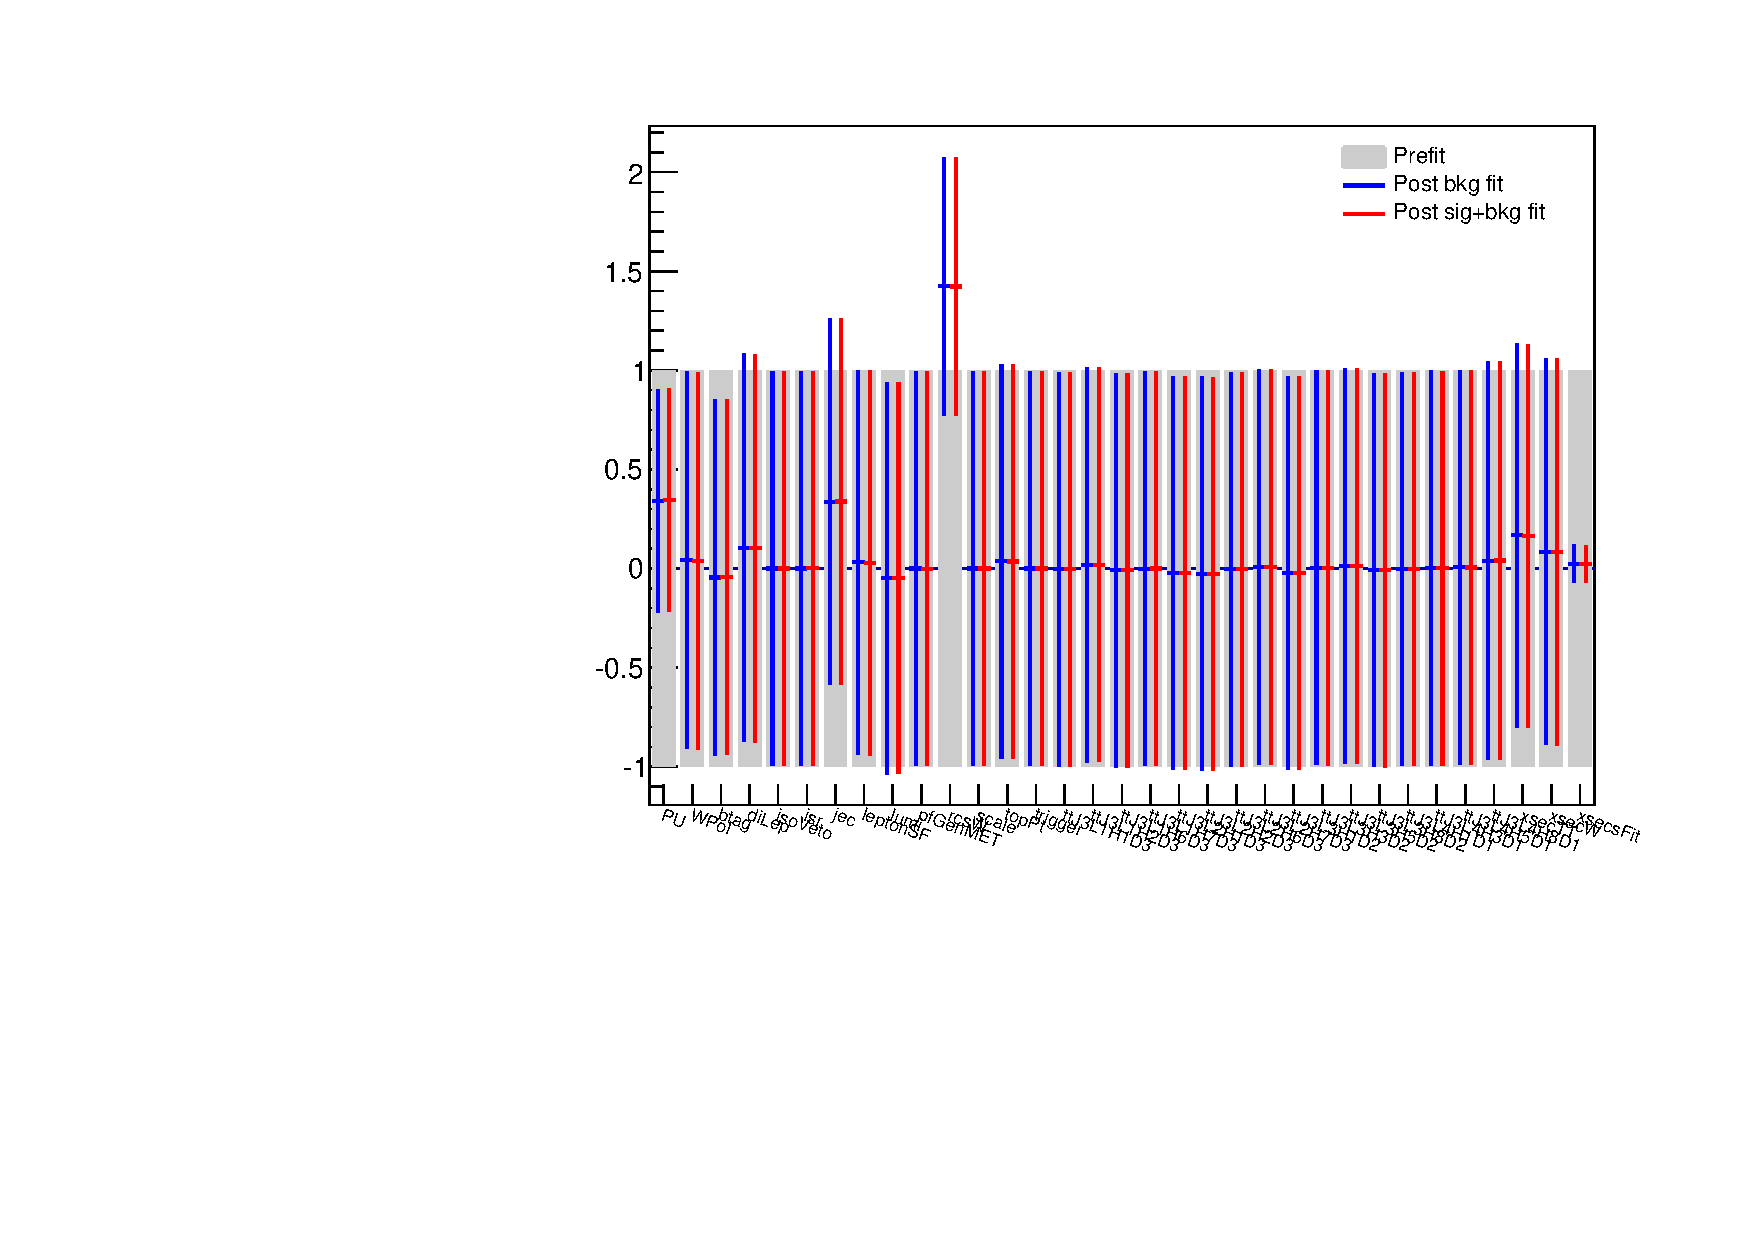
\includegraphics[width=0.5\textwidth]{Plots/nuisances/nuisances-other.pdf}}\\
\subfigure[$\kappa$ parameters]{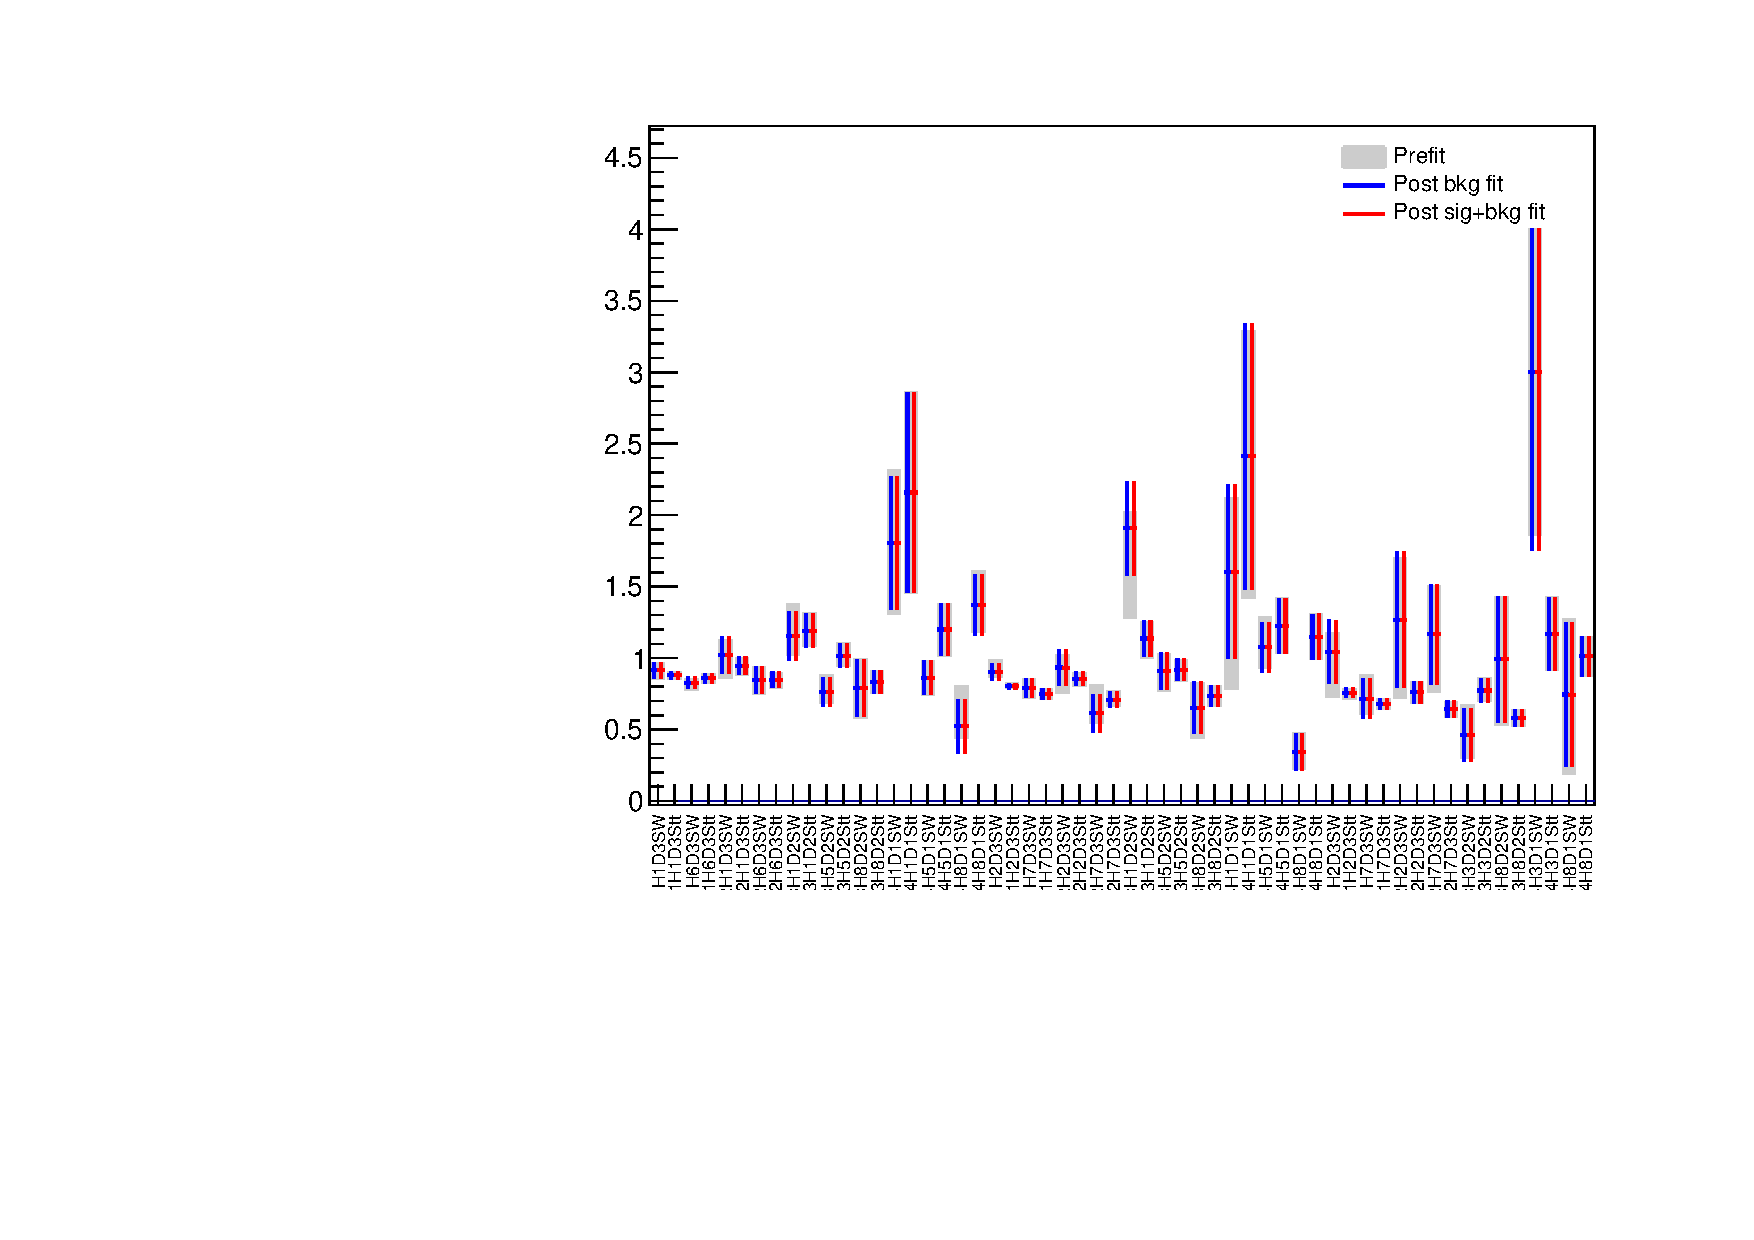
\includegraphics[width=0.5\textwidth]{Plots/nuisances/nuisances-kJ.pdf}} \\
\subfigure[QCD estimate]{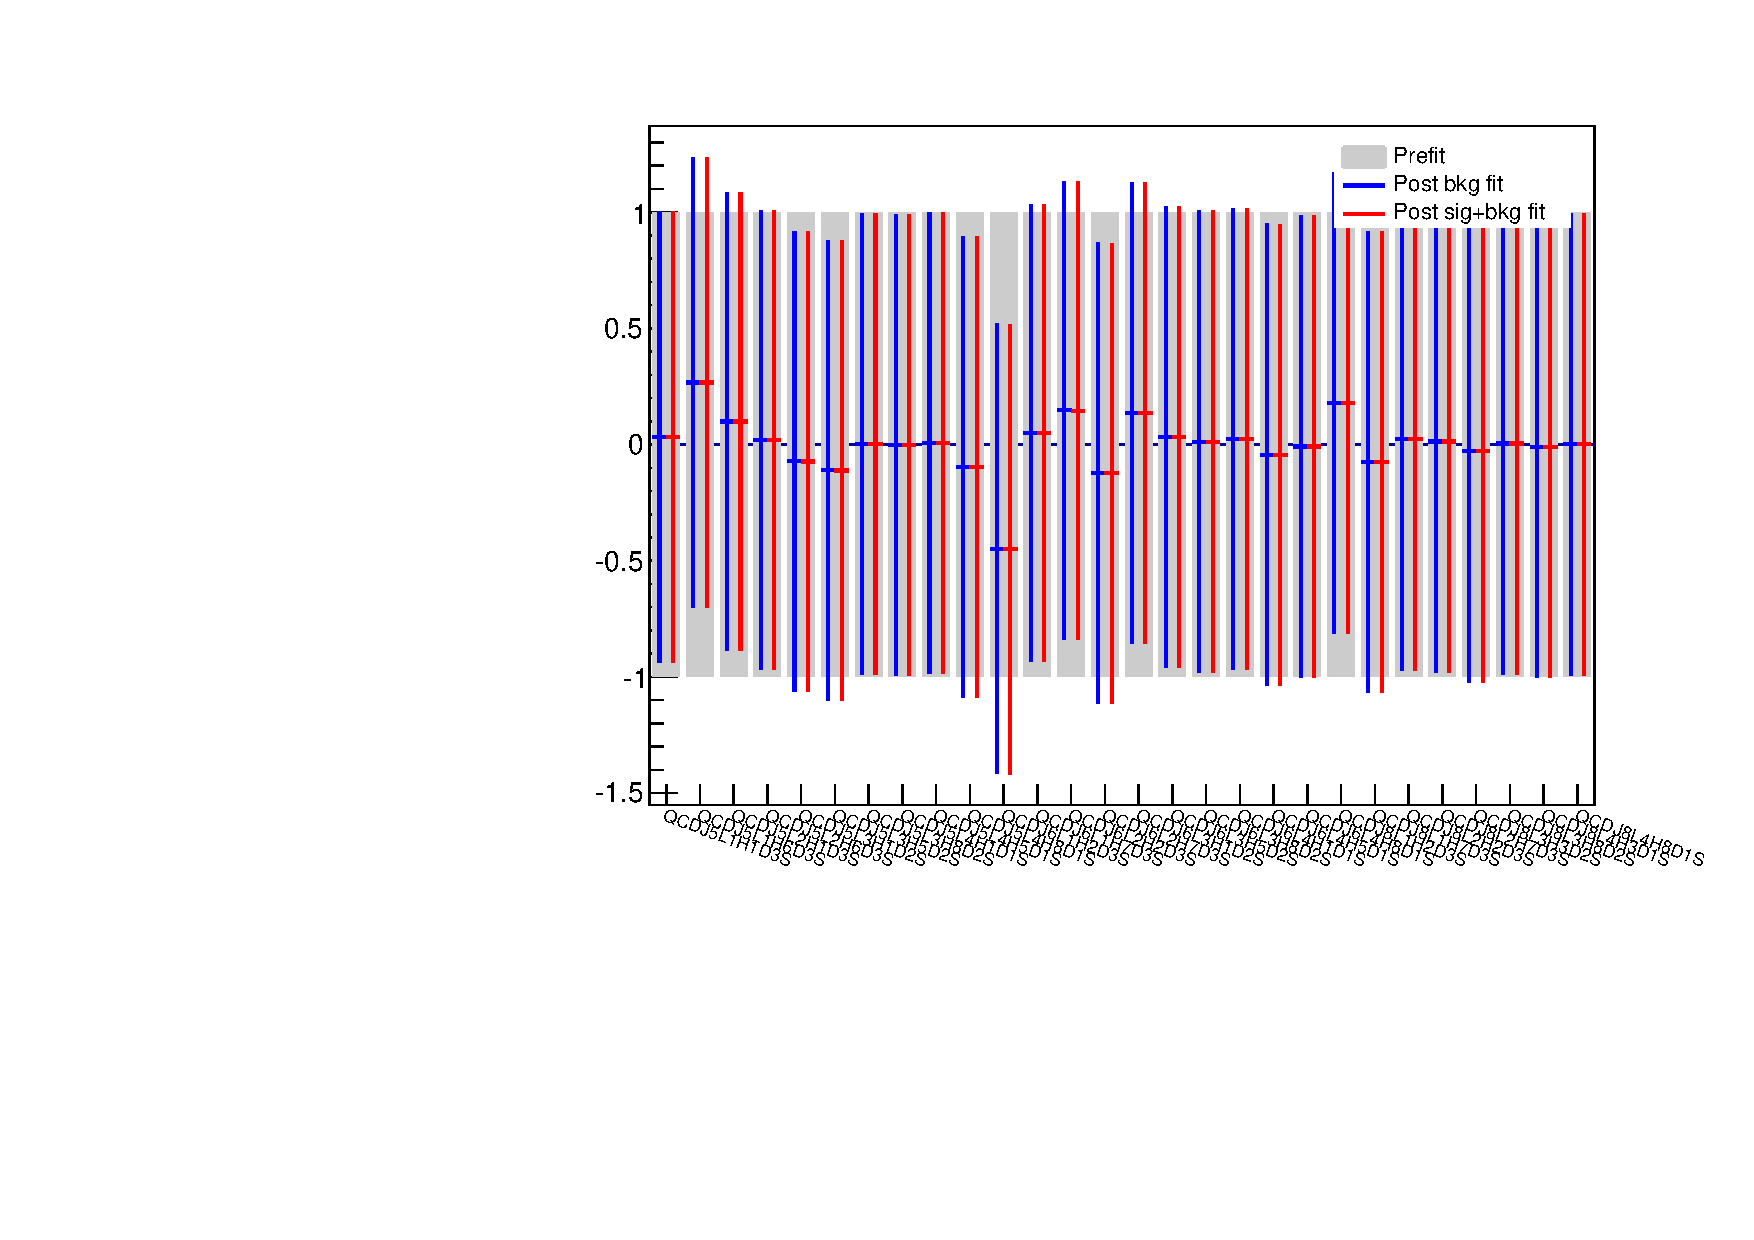
\includegraphics[width=0.5\textwidth]{Plots/nuisances/nuisances-QCD.pdf}}\\
\end{center}
\caption{Prefit (grey), s+b postfit (red) and, b-only postfit (blue) values of nuisance parameters included in the fit. }
\label{fig:nuisances1}
\end{figure}

\begin{figure}[!hbtp]
\begin{center}
\subfigure[nuisances in $W$ Side Band]{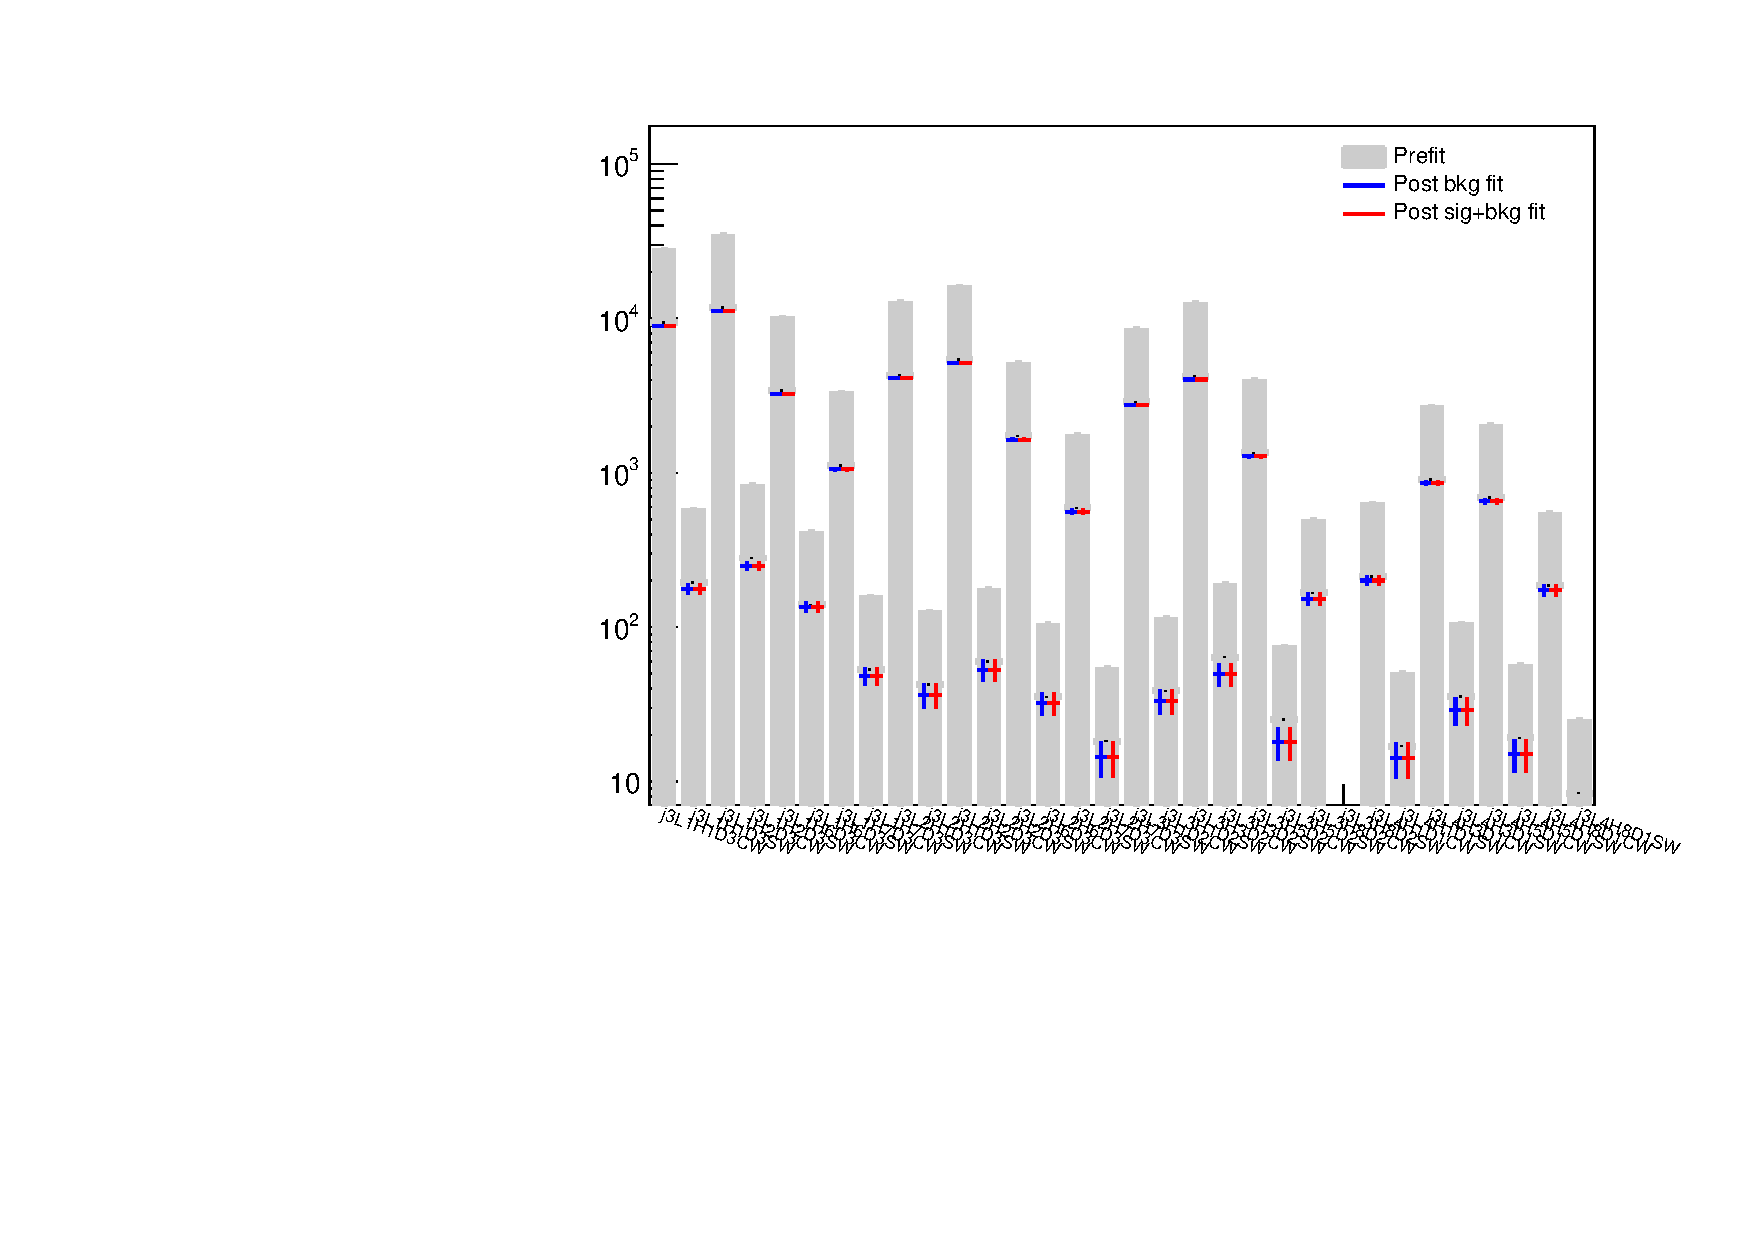
\includegraphics[width=0.5\textwidth]{Plots/nuisances/nuisances-j3.pdf}} \\
\subfigure[nuisances in $\ttbar$ Side Band]{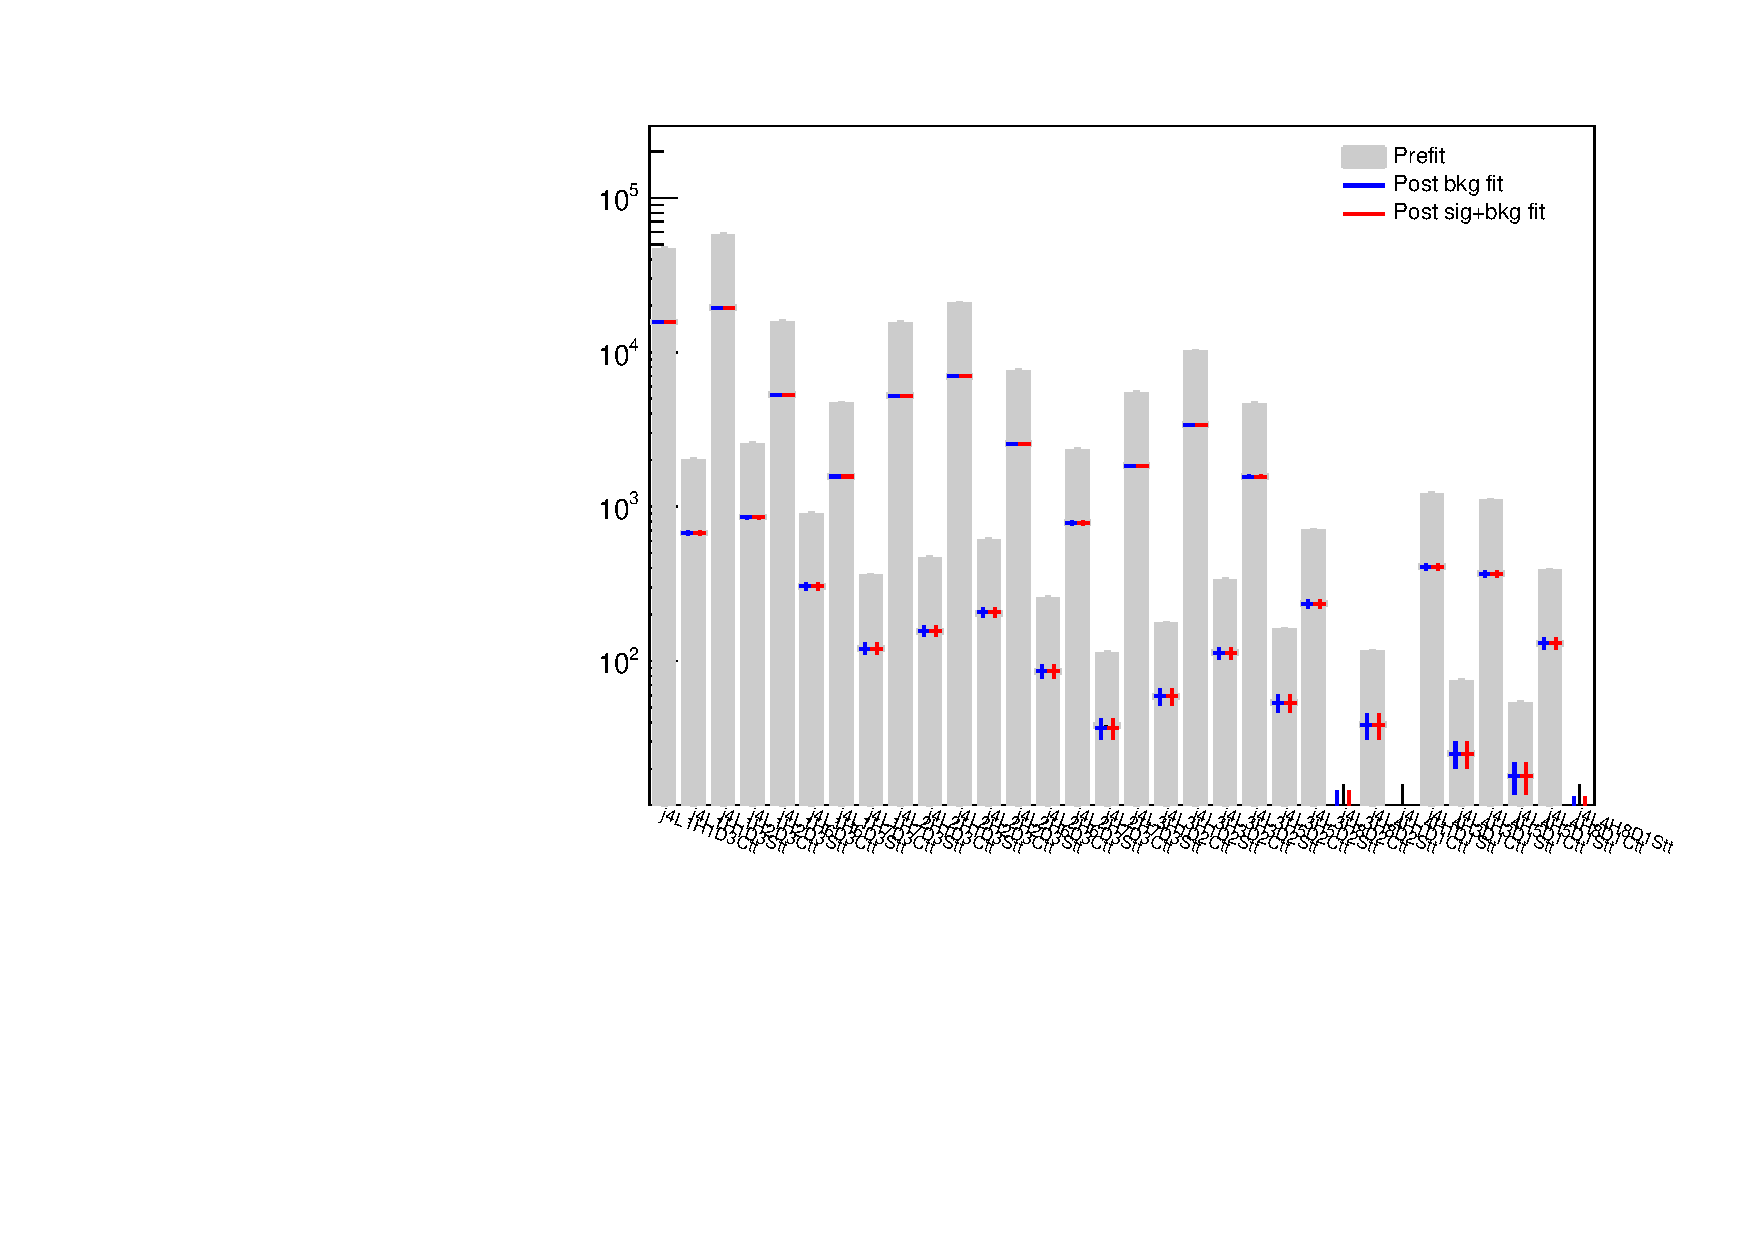
\includegraphics[width=0.5\textwidth]{Plots/nuisances/nuisances-j4.pdf}} \\
\end{center}
\caption{Prefit (grey), s+b postfit (red) and, b-only postfit (blue) values of nuisance parameters in side band regions included in the fit. }
\label{fig:nuisances2}
\end{figure}